	%%% LaTeX Template: Designer's CV
%%%
%%% Source: http://www.howtotex.com/
%%% Feel free to distribute this template, but please keep the referal to HowToTeX.com.
%%% Date: March 2012


%%%%%%%%%%%%%%%%%%%%%%%%%%%%%%%%%%%%%
% Document properties and packages
%%%%%%%%%%%%%%%%%%%%%%%%%%%%%%%%%%%%%
\documentclass[a4paper,11pt,final]{memoir}

% misc
\renewcommand{\familydefault}{bch}	% font
\pagestyle{empty}					% no pagenumbering
\setlength{\parindent}{0pt}			% no paragraph indentation

\usepackage[T1]{fontenc}
\usepackage[utf8]{inputenc}
% required packages (add your own)
\usepackage{flowfram}										% column layout
\usepackage[top=1cm,left=1cm,right=1cm,bottom=1cm]{geometry}% margins
\usepackage{graphicx}										% figures
\usepackage{url}											% URLs
\usepackage[usenames,dvipsnames]{xcolor}					% color
\usepackage{multicol}										% columns env.
	\setlength{\multicolsep}{0pt}
\usepackage{paralist}										% compact lists
\usepackage[super]{nth}
\usepackage{tikz}
\usepackage{hyperref}
\hypersetup{colorlinks,citecolor=black,filecolor=black,linkcolor=black,urlcolor=black} % pour mettre les liens en noirs, sans cadre
\usepackage[english]{babel}

\definecolor{dark_gray}{rgb}{0.3,0.3,0.3}

%%%%%%%%%%%%%%%%%%%%%%%%%%%%%%%%%%%%%
% Create column layout
%%%%%%%%%%%%%%%%%%%%%%%%%%%%%%%%%%%%%
% define length commands
\setlength{\vcolumnsep}{\baselineskip}
\setlength{\columnsep}{\vcolumnsep}

% frame setup (flowfram package)
% left frame
\newflowframe{0.27\textwidth}{\textheight}{0pt}{0pt}[left]
	\newlength{\LeftMainSep}
	\setlength{\LeftMainSep}{0.26\textwidth}
	\addtolength{\LeftMainSep}{1\columnsep}

% small static frame for the vertical line
\newstaticframe{1.5pt}{\textheight}{\LeftMainSep}{0pt}

% content of the static frame
\begin{staticcontents}{1}
\hfill
\tikz{%
	\draw[loosely dotted,color=RoyalBlue,line width=1.5pt,yshift=0]
	(0,0) -- (0,\textheight);}%
\hfill\mbox{}
\end{staticcontents}

% right frame
\addtolength{\LeftMainSep}{1.5pt}
\addtolength{\LeftMainSep}{1\columnsep}
\newflowframe{0.68\textwidth}{\textheight}{\LeftMainSep}{0pt}[main01]


%%%%%%%%%%%%%%%%%%%%%%%%%%%%%%%%%%%%%
% define macros (for convience)
%%%%%%%%%%%%%%%%%%%%%%%%%%%%%%%%%%%%%
\newcommand{\Sep}{\vspace{1.5em}}
\newcommand{\SmallSep}{\vspace{0.5em}}

\newenvironment{AboutMe}
	{\ignorespaces%\textbf{\color{RoyalBlue} About me}}
}
	{\Sep\ignorespacesafterend}

\newcommand{\CVSection}[1]
	{\Large\textbf{#1}\par
	\SmallSep\normalsize\normalfont}

\newcommand{\CVItem}[2]
	{\textbf{\color{RoyalBlue} #1 \color{dark_gray} #2}\normalsize\normalfont}

\newcommand{\city}[1]
	{{\small\color{dark_gray}\emph{#1}}\normalsize\normalfont}

\newcommand{\SkillSection}[1]
	{\normalsize{\textbf{#1\\}}\normalfont\small}%\footnotesize}

\newcommand{\SkillItem}[1]
{\vspace{0.25em}\textbf{\color{RoyalBlue} #1}\normalfont}

%%%%%%%%%%%%%%%%%%%%%%%%%%%%%%%%%%%%%
% Begin document
%%%%%%%%%%%%%%%%%%%%%%%%%%%%%%%%%%%%%
\begin{document}

% Left frame
%%%%%%%%%%%%%%%%%%%%
% Photo
\begin{figure}
	\hfill
	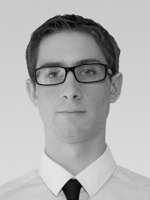
\includegraphics[width=0.5\columnwidth]{../IMG_7936-Modifier_cv}
	\vspace{-0.5cm}
\end{figure}

% Personnal Infos
\begin{flushright}\small
	Le Genestel\\
	50700 Valognes\\
	France\\
	{\href{mailto:rom.reignier@gmail.com}{\nolinkurl{rom.reignier@gmail.com}}}\\
	+33 6 09 52 16 18\\
	23 years old\\
	Driving License
\end{flushright}%\normalsize

\begin{flushleft}
% Engineering
\SkillSection{Engineering}
%Mechnanics\\
Design of Systems\\
CAD \& CAM\\
%Analysis of mechanisms\\
Resistance of the materials\\
%Materials\\
Electronics\\
Digital methods\\
%Algorithmic\\
%Database\\
%Thermal transferts\\
Automatics\\
%Servo-systems\\
Robotics\\
%Communication\\
Computer Vision
\SmallSep

% Computer Skills
\SkillSection{Computer Skills}
\vspace{-0.25em}
%\SkillItem{Mathematics}
%Matlab, Maple\\
\SkillItem{Programming}\\
C, C++, Python, Matlab, Simulink, LabView, Java, OpenCV, Qt, Git\\
\SkillItem{Embedded}\\
Robot Operating System (ROS), GNU/Linux (Kernel driver, Yocto, Buildroot), Arduino, AVR, dsPIC, ARM, mbed\\
\SkillItem{CAD}\\
CATIA V5, SolidWorks, ADAMS\\
\SkillItem{Web Development}\\
HTML5, CSS3, PHP, MySQL\\
\SkillItem{Office Automation Programs}\\
Word, Excel (Visual Basic), PowerPoint, Access, Project, \LaTeX\\
%\SkillItem{Image Editing}\\
%Photoshop, Lightroom, Illustrator, Gimp, Inkscape, FinalCut Pro X\\
\SmallSep

% Languages
\SkillSection{Languages}
\vspace{-0.25em}
\SkillItem{English}: Advanced level\\
(TOEIC: 920 pts)\\
\SkillItem{Spanish}: Baccalaureat level\\
\SkillItem{German}: Basic
\SmallSep

% Sports
\SkillSection{Sports}
Cycling, road \& MTB\\
Running\\
%Swimming
\SmallSep

% Hobbies
\SkillSection{Hobbies}
Robotics\\
Electronics\\
Mechanics\\
Gardening / Farming\\
Photography\\
%General mechanics\\
First level diploma in aeronautics\SmallSep

% Travels
\SkillSection{Travels}
Malaysia, Singapore, Togo
InterRail 2014 : Amsterdam, Berlin, Prague, Vienna, Geneva
%Netherlands, Germany, Czech Republic, Austria, Switzerland
\end{flushleft}
\framebreak


% Right frame
%%%%%%%%%%%%%%%%%%%%
%\Huge\bfseries {\color{RoyalBlue} Romain \textsc{Reignier}} \\
\Huge\bfseries {\color{RoyalBlue} Romain REIGNIER} \\
\Large\bfseries Mechatronics \& Robotics Supméca Engineer\\
% About me
%\begin{AboutMe}
%\end{AboutMe}

% Experience
\CVSection{Experience}
\CVItem{March 2015 -- August 2015,}{CEA} -- \city{Marcoule, Languedoc-Rousillon}\\
Engineer internship: Implementation of ROS and the Gazebo simulator on a hexapod robot. Developpment in C++ of a new gait for uneven terrain to be used for investigation in nuclear dismantling.\SmallSep

\CVItem{October 2014 -- February 2015}{Supméca} -- \city{La Garde, PACA}\\
\nth{3} year projects:\\
-- Design study of a mobile manipulator robot for nuclear sanitation in partnership with the CEA.\\
-- Sensors implementation in a vacuum cleaner to monitor the energy consumption on an Android app via Bluetooth LE for the LISSMA laboratory.\SmallSep

\CVItem{April 2014 -- June 2015}{Supméca} -- \city{La Garde, PACA}\\
\nth{2} year project: Upgrade of a pneumatic PLC installation. Mechanics and Grafcet \& Ladder programming.
\SmallSep

\CVItem{September 2013 -- January 2014,}{R\&D CLAAS Tractor} -- \city{Vélizy, Île-de-France}\\
Assistant engineer internship: Work with the HVAC expert on the project to improve the AC in the cabin of the tractors.
Analysis of data from simulations and tests, design optimizations then prepare industrialization.
\SmallSep

\CVItem{January 2013,}{DCNS} -- \city{Cherbourg, Normandy}\\
Operator internship: Work with numerical machine tools (milling, boring machines and lathe) in the construction workshop of French nuclear submarines.\SmallSep

\CVItem{2006 -- 2012}{}\\
Various jobs: Deauville International Polo Club, EPR construction site for Électricité de France, appliances maintenance, machining operations, farming.
\Sep

\CVSection{Projects \& Associations}
\CVItem{Robotics club of Supmeca}{}Conception, making and programming of robots for French Robotics Cup (Eurobot) 2013, 2014 and 2015.
\SmallSep

\CVItem{Supwave}{}Supervisor of the electronics in an autonomous sailboat.
\SmallSep

\CVItem{Aerocorp}{}Manager for the electronics of a radio-controlled model aircraft.\SmallSep

\CVItem{Supmeca Sans Frontières}{}Humanitarian association which has the aim of bringing water to a Togolese orphanage.
\SmallSep

\CVItem{Scouts et Guides de France}{}Boyscout for 8 years.
Chief on a summer camp in 2012 and Humanitarian project in Togo in August 2013.
\Sep

% Education
\CVSection{Education}
\CVItem{2012 -- 2015,}{Supméca Engineering School} -- \city{La Garde, PACA}\\
\emph{Institut Supérieur de Mécanique de Paris} (ex CESTI)\\
A selective Mechanical Engineering school,\\
Major in \textbf{Robotics and Mecatronics Systems}.
%An engineering course focusing in mechanics with Robotics and Mecatronics specialisation.
\SmallSep

\CVItem{2014 -- 2015,}{University of Toulon} -- \city{La Garde, PACA}\\
Master of Sciences in Physics and Engineering Sciences,\\
Specialization in \textbf{Vision and Control}.
%Image Processing, Vision, Detection, Pattern Recognition, Motion Planning.
\SmallSep

\CVItem{2009 -- 2012,}{CPGE Victor Hugo} -- \city{Caen, Normandy}\\
Highly selective classes to prepare for the competitive exams to the Grandes Ecoles. Physics and Sciences of Engineer.
%Highly selective classes to prepare for the competitive exams\\
%to the Grandes Ecoles.
%\SmallSep
%\CVItem{2006 -- 2009,}{Scientific Baccalaureat} -- \city{Valognes, Normandy}\\
%Secondary School diploma in Sciences, specialized in Physics.
%With Honors.
\Sep

%%%%%%%%%%%%%%%%%%%%%%%%%%%%%%%%%%%%%
% End document
%%%%%%%%%%%%%%%%%%%%%%%%%%%%%%%%%%%%%
\end{document}
